\documentclass{article}
\usepackage{fancyhdr}
\usepackage{ctex}
\usepackage{listings}
\usepackage{graphicx}
\usepackage[a4paper, body={18cm,22cm}]{geometry}
\usepackage{amsmath,amssymb,amstext,wasysym,enumerate,graphicx}
\usepackage{float,abstract,booktabs,indentfirst,amsmath}
\usepackage{array}
\usepackage{booktabs}
\usepackage{multirow}
\usepackage{url}
\usepackage{diagbox}
\renewcommand\arraystretch{1.4}
\usepackage{indentfirst}
\setlength{\parindent}{2em}
\usepackage{enumitem}
\setmonofont{DejaVu Sans Mono}
\usepackage{listings}
\usepackage{xcolor}
\usepackage{makecell}
\setCJKmonofont{黑体}
\usepackage{tikz}
\usepackage{tabularx}
\usepackage{amsmath}
\usetikzlibrary{positioning, arrows.meta}
\lstset{
    % language = C,
    xleftmargin = 3em,xrightmargin = 3em, aboveskip = 1em,
	backgroundcolor = \color{white}, % 背景色
	basicstyle = \small\ttfamily, % 基本样式 + 小号字体
	rulesepcolor= \color{gray}, % 代码块边框颜色
	breaklines = true, % 代码过长则换行
	numbers = left, % 行号在左侧显示
	numberstyle = \small, % 行号字体
    numbersep = -14pt, 
    keywordstyle=\color{purple}\bfseries, % 关键字颜色
    commentstyle =\color{red!50!green!50!blue!60}, % 注释颜色
    stringstyle = \color{red}, % 字符串颜色
    morekeywords={ASSERT, int64_t, uint32_t},
	frame = shadowbox, % 用(带影子效果)方框框住代码块
	showspaces = false, % 不显示空格
	columns = fixed, % 字间距固定
} 
\lstset{
    sensitive=true,
    moreemph={ASSERT, NULL}, emphstyle=\color{red}\bfseries,
    moreemph=[2]{int64_t, uint32_t, tid_t, uint8_t, int16_t, uint16_t, int32_t, size_t}, emphstyle=[2]\color{purple}\bfseries,
    }
%--------------------页眉--------------------%
\pagestyle{fancy}
\fancyhead[L]{}
\fancyhead[R]{}
\fancyhead[C]{华东师范大学软件工程学院实验报告}
\fancyfoot[C]{-\thepage-}
\renewcommand{\headrulewidth}{1.5pt}
%--------------------标题--------------------%
\begin{document}
\begin{center}
  \LARGE{{\textbf{\heiti 华东师范大学软件工程学院实验报告}}}
  \begin{table}[H]
    \centering
    \begin{tabular}{p{2cm}p{4cm}<{\centering}p{1cm}p{2cm}p{4cm}<{\centering}}
      实验课程:    & 计算机网络 & \quad & 年\qquad 级: & 2022级      \\ \cline{2-2} \cline{5-5}
      实验编号:    & Lab 06     & \quad & 实验名称:    & TCP
      \\ \cline{2-2} \cline{5-5}
      姓\qquad 名: & 李鹏达     & \quad & 学\qquad 号: & 10225101460 \\ \cline{2-2} \cline{5-5}
    \end{tabular}
  \end{table}
\end{center}
\rule{\textwidth}{1pt}
%--------------------正文--------------------%
\section{实验目的}
\begin{enumerate}[noitemsep, label={{\arabic*})}]
  \item 学会通过 \texttt{Wireshark}获取 \texttt{TCP}消息
  \item 掌握 \texttt{TCP}数据包结构
  \item 掌握 \texttt{TCP}数据包各字段的含义
  \item 掌握 \texttt{TCP}连接建立和释放的步骤
  \item 掌握 \texttt{TCP}数据传输阶段的过程
\end{enumerate}
\section{实验内容与实验步骤}
\subsection{实验内容}

\subsubsection{捕获 \texttt{TCP} 报文}

\begin{enumerate}[noitemsep]
  \item 以 \url{http://img.zcool.cn/community/01dcd059117b12a801216a3e9c4fd5.jpg@1280w_1l_2o_100sh.jpg}为例,用 \texttt{wget}确认该链接有效
  \item 启动\texttt{Wireshark},在菜单栏的捕获 \( \to \) 选项中进行设置,选择已连接的以太网,设置捕获过滤器为\texttt{tcp and host img.zcool.cn}。我们主要观察客户端与服务器之间的\texttt{tcp}流。
  \item 捕获开始后,重复第一步,重新发送请求。
  \item 当\texttt{wget}命令结束后,停止\texttt{Wireshark}捕获。
\end{enumerate}

\subsubsection{分析 \texttt{TCP} 报文}

要求:
\begin{enumerate}[noitemsep]
  \item 画出\texttt{TCP}数据报的结构图
  \item 分析\texttt{TCP}数据报头各字段作用
\end{enumerate}

\subsubsection{\texttt{TCP} 连接的建立和释放}

TCP的三次握手协议主要分为以下三个步骤:
\begin{enumerate}[noitemsep]
  \item 客户端发送一个\texttt{SYN}包给服务器,然后等待应答。
  \item 服务器端回应给客户端一个\texttt{ACK=1}、\texttt{SYN=1}的\texttt{TCP}数据段。
  \item 客户必须再次回应服务器端一个\texttt{ACK}确认数据段。
\end{enumerate}

回答问题:
\begin{enumerate}[noitemsep]
  \item 观察客户端与服务器的连接建立过程,画出三次握手协议的步骤图
  \item 观察并分析\texttt{TCP}数据段中的\texttt{option}字段
\end{enumerate}

TCP的四次挥手主要分为以下四个步骤:
\begin{enumerate}[noitemsep]
  \item 客户端进程发出断开连接指令,这将导致客户端的\texttt{TCP}程序创建一个特殊的\texttt{TCP}报文段,发送到服务器。这个报文段的\texttt{FIN}字段被置为1,表示这是一条断开连接的报文;
  \item 服务器接收到客户端发来的断开连接报文,向客户端回送这个报文的确认报文(\texttt{ACK}字段为1),告诉服务器已经接收到\texttt{FIN}报文,并允许断开连接;
  \item 服务器发送完确认报文后,服务器的\texttt{TCP}程序创建一条自己的断开连接报文,此报文的\texttt{FIN}字段被置为1,然后发往客户端;
  \item 客户端接收到服务器发来的\texttt{FIN}报文段,则产生一条确认报文(\texttt{ACK}为1),发送给服务器,告知服务器已经接收到了它的断开报文。服务器接收到这条\texttt{ACK}报文段后,释放\texttt{TCP}连接相关的资源(缓存和变量),而客户端等待一段时间后(半分钟、一分钟或两分钟),也释放处于客户端的缓存和变量。
\end{enumerate}

回答问题:
\begin{enumerate}[noitemsep]
  \item 观察客户端与服务器连接的释放过程,画出释放连接的步骤图
  \item 思考为什么连接的时候是三次握手,关闭的时候却是四次挥手?
\end{enumerate}

\subsubsection{TCP 数据传输}

观察Wireshark生成的IO图表

回答问题:(以各自实验为准)
\begin{enumerate}[label={\arabic*)}, noitemsep]
  \item 实验中的下载速率是多少? \texttt{Bits/s} \& \texttt{packets/s}
  \item 实验中的上传速率,即ACK消息的发送速率是多少? \texttt{Bits/s} \& \texttt{packets/s}
\end{enumerate}

观察数据包传输过程

\begin{enumerate}[noitemsep]
  \item 观察数据传输过程中 \texttt{Acknowledgment number},\texttt{sequence number} 和 \texttt{Segment Len} 之间的变化
  \item 如果最近从服务器收到的 \texttt{TCP} 数据段的序列号是 $X$,那么下一个发送的 \texttt{ACK} 是多少?
\end{enumerate}

\subsubsection{问题讨论}

\begin{enumerate}[noitemsep]
  \item Explore the congestion control and the classic AIMD behavior of TCP. To do this, you will likely want to capture a trace while you are sending (not receiving) a moderate amount of data on a TCP connection. You can then use the “TCP Stream Graph” tools as well as other analysis to observe how the congestion window changes over time.
  \item Explore the reliability mechanisms of TCP more deeply. Capture a trace of a connection that includes segment loss. See what triggers the retransmissions and when. Also look at the round-trip time estimator.
  \item Look at the use of options including SACK to work through the details. You should see information about ranges of received bytes during times of segment loss.
  \item TCP is the transport layer underlying the web. You can see how your browser makes use of TCP by setting up concurrent connections.
\end{enumerate}


\subsection{实验步骤}

\begin{enumerate}[noitemsep]
  \item 以 \url{http://img.zcool.cn/community/01dcd059117b12a801216a3e9c4fd5.jpg}为例,用 \texttt{wget}确认该链接有效
        \begin{lstlisting}
    PS> wget http://img.zcool.cn/community/01dcd059117b12a801216a3e9c4fd5.jpg
  \end{lstlisting}
  \item 启动\texttt{Wireshark},在菜单栏的捕获 \( \to \) 选项中进行设置,选择已连接的以太网,设置捕获过滤器为\texttt{tcp and host img.zcool.cn}。我们主要观察客户端与服务器之间的\texttt{tcp}流。
  \item 捕获开始后,重复第一步,重新发送请求。
  \item 当\texttt{wget}命令结束后,停止\texttt{Wireshark}捕获。
  \item 分析 \texttt{TCP} 报文
\end{enumerate}

\section{实验环境}


\begin{itemize}[noitemsep]
  \item 操作系统:\texttt{Windows 11 家庭中文版 23H2 22631.2715}
  \item 网络适配器:\texttt{Killer(R) Wi-Fi 6 AX1650i 160MHz Wireless Network Adapter(201NGW)}
  \item \texttt{Wireshark}:\texttt{Version 4.2.0 (v4.2.0-0-g54eedfc63953)}
  \item \texttt{wget}:\texttt{GNU Wget 1.21.4 built on mingw32}
\end{itemize}


\section{实验结果与分析}

\subsection{捕获 \texttt{TCP} 报文}

首先,我们使用 \texttt{wget} 确认链接有效。

\begin{figure}[H]
  \centering
  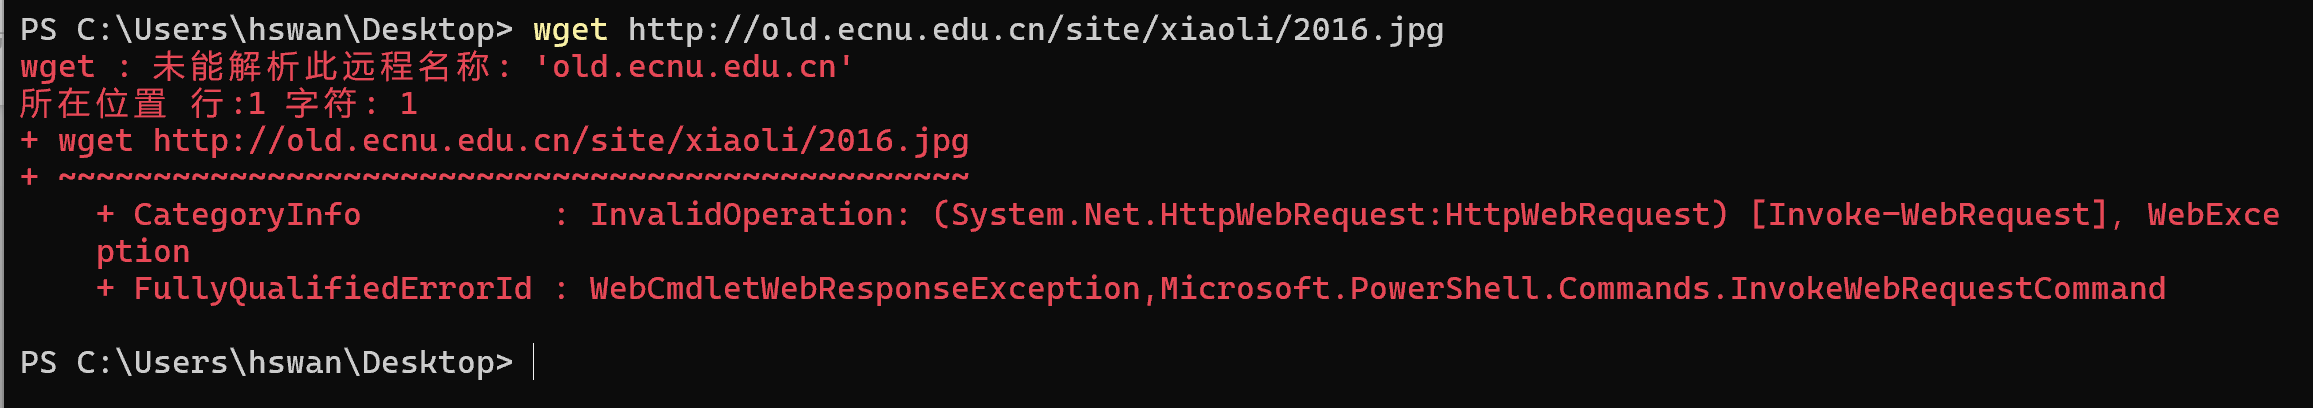
\includegraphics[width=0.8\textwidth]{img/1.png}
  \caption{使用 \texttt{wget} 确认链接有效}
\end{figure}

然后,我们启动\texttt{Wireshark},在菜单栏的捕获 \( \to \) 选项中进行设置,选择已连接的以太网,设置捕获过滤器为\texttt{tcp and host img.zcool.cn}。我们主要观察客户端与服务器之间的\texttt{tcp}流。

\begin{figure}[H]
  \centering
  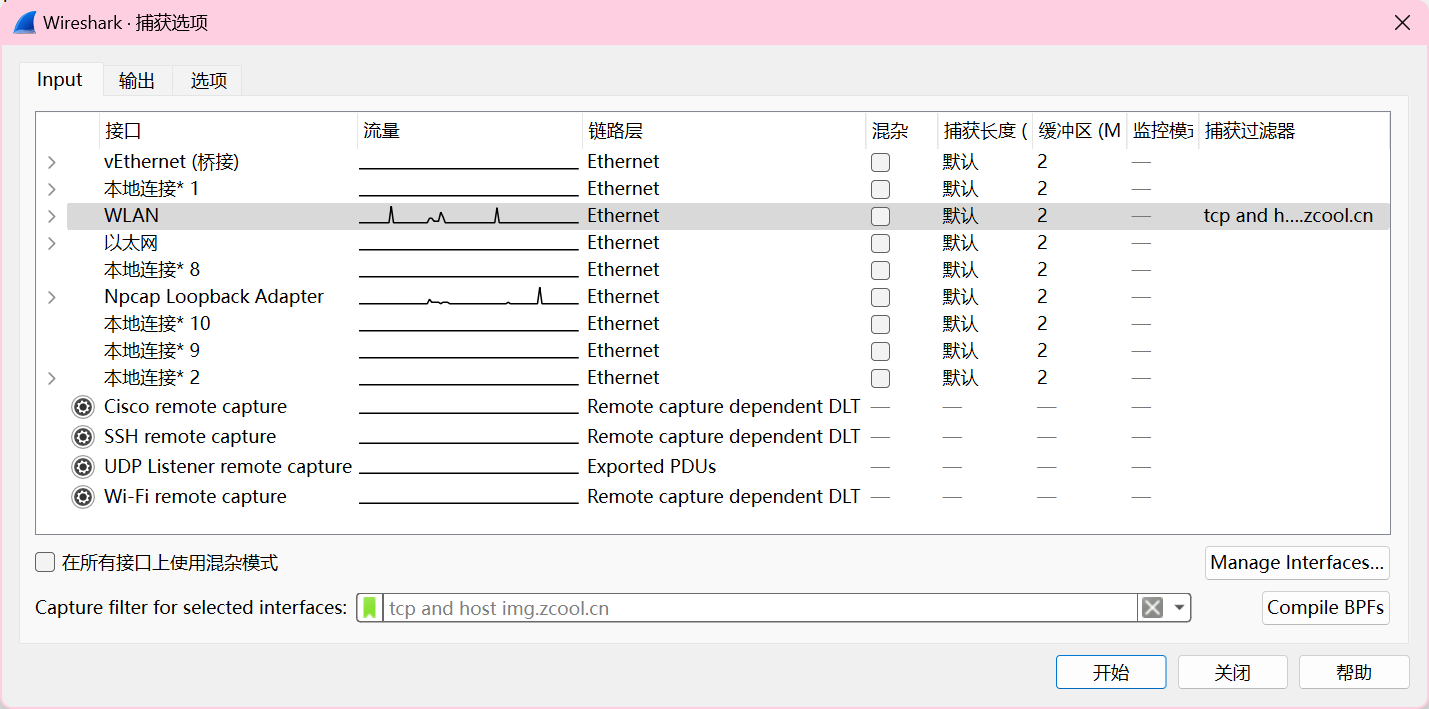
\includegraphics[width=0.8\textwidth]{img/2.png}
  \caption{设置捕获过滤器}
\end{figure}

捕获开始后,重复第一步,重新发送请求。

\begin{figure}[H]
  \centering
  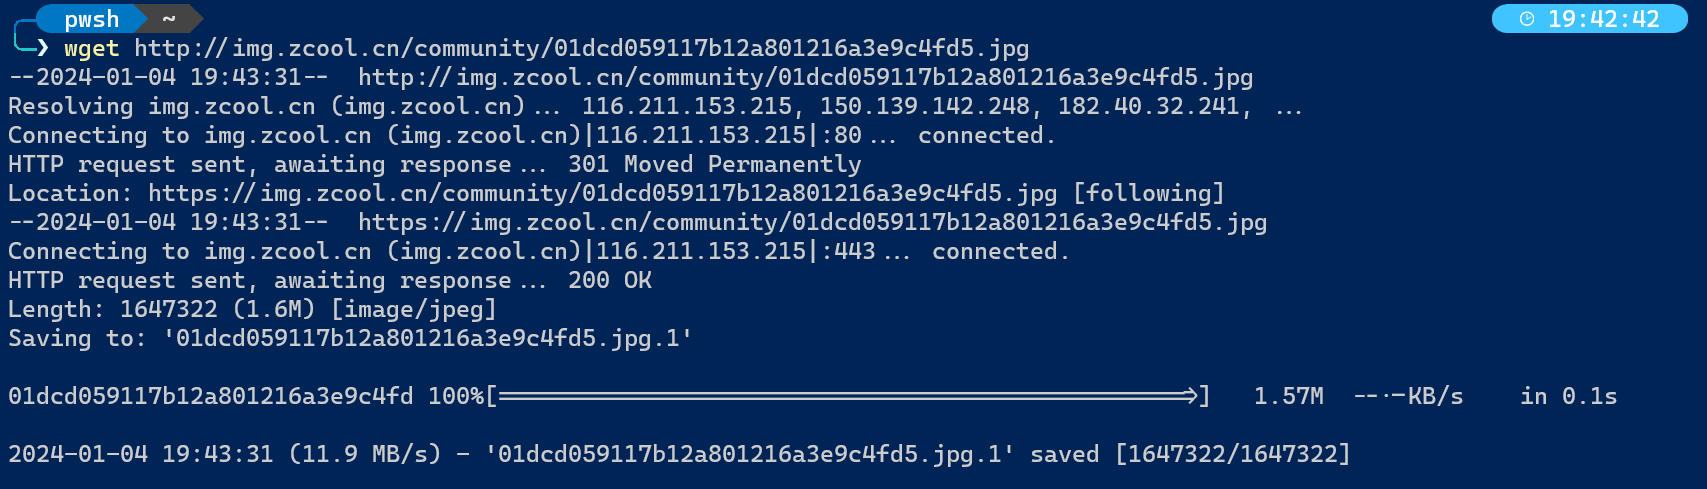
\includegraphics[width=0.8\textwidth]{img/3.png}
  \caption{重新发送请求}
\end{figure}

当\texttt{wget}命令结束后,停止\texttt{Wireshark}捕获。
捕获结果如下:

\begin{figure}[H]
  \centering
  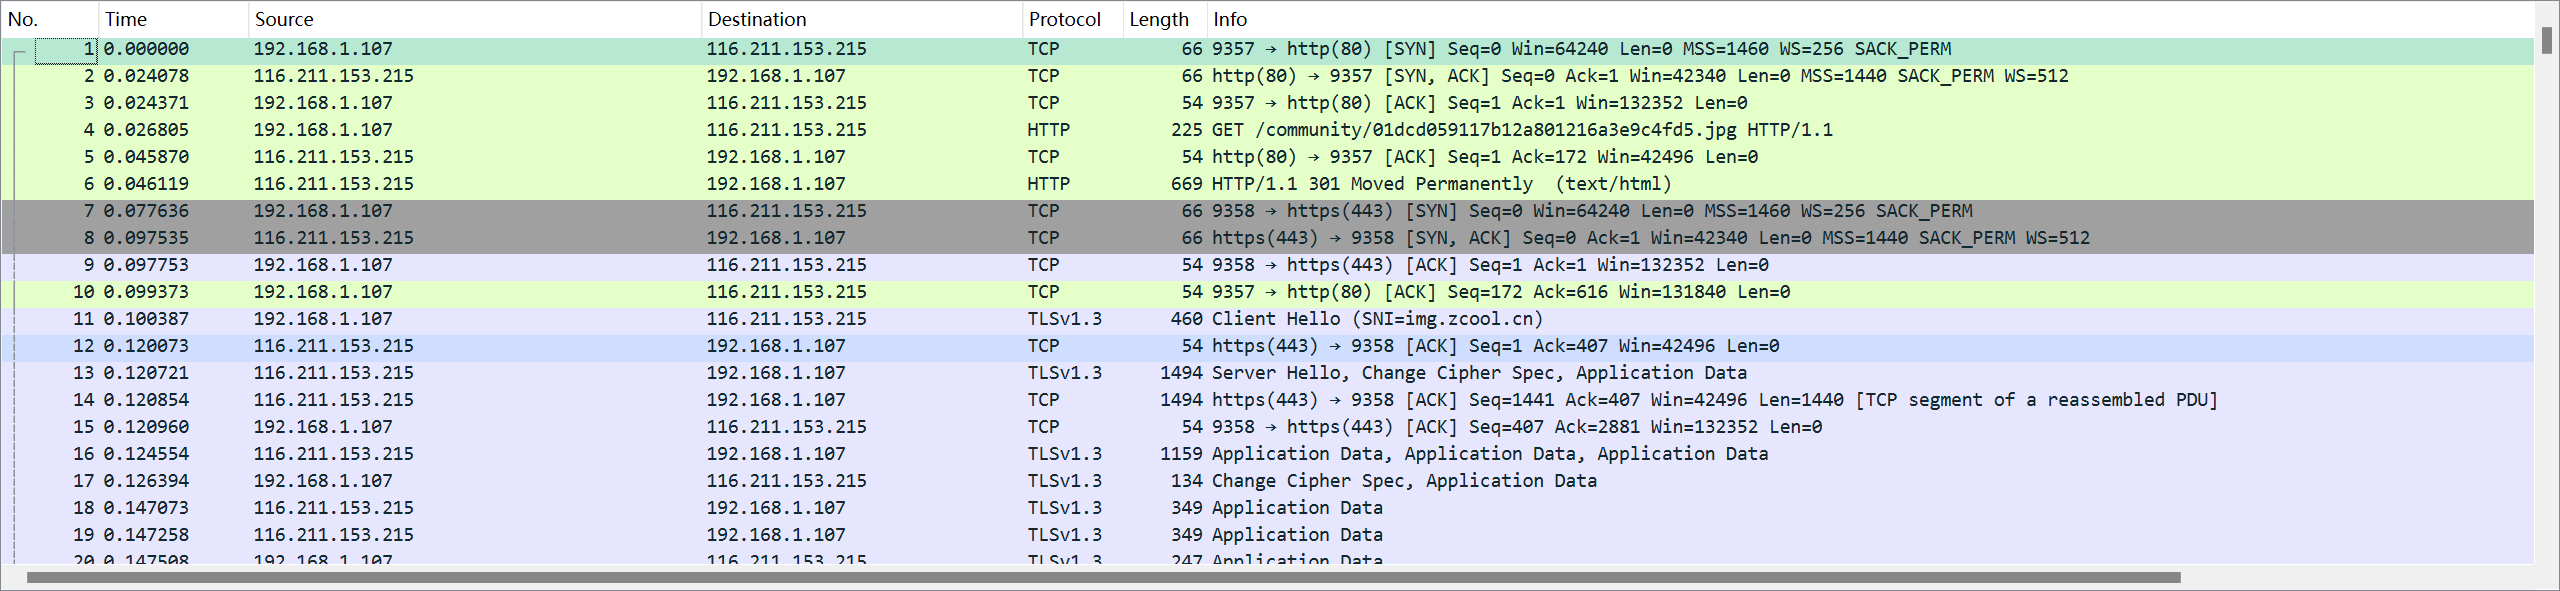
\includegraphics[width=0.8\textwidth]{img/4.png}
  \caption{捕获结果}
\end{figure}


\subsection{分析 \texttt{TCP} 报文}

选择一个\texttt{TCP}数据包,如下所示:

\begin{figure}[H]
  \centering
  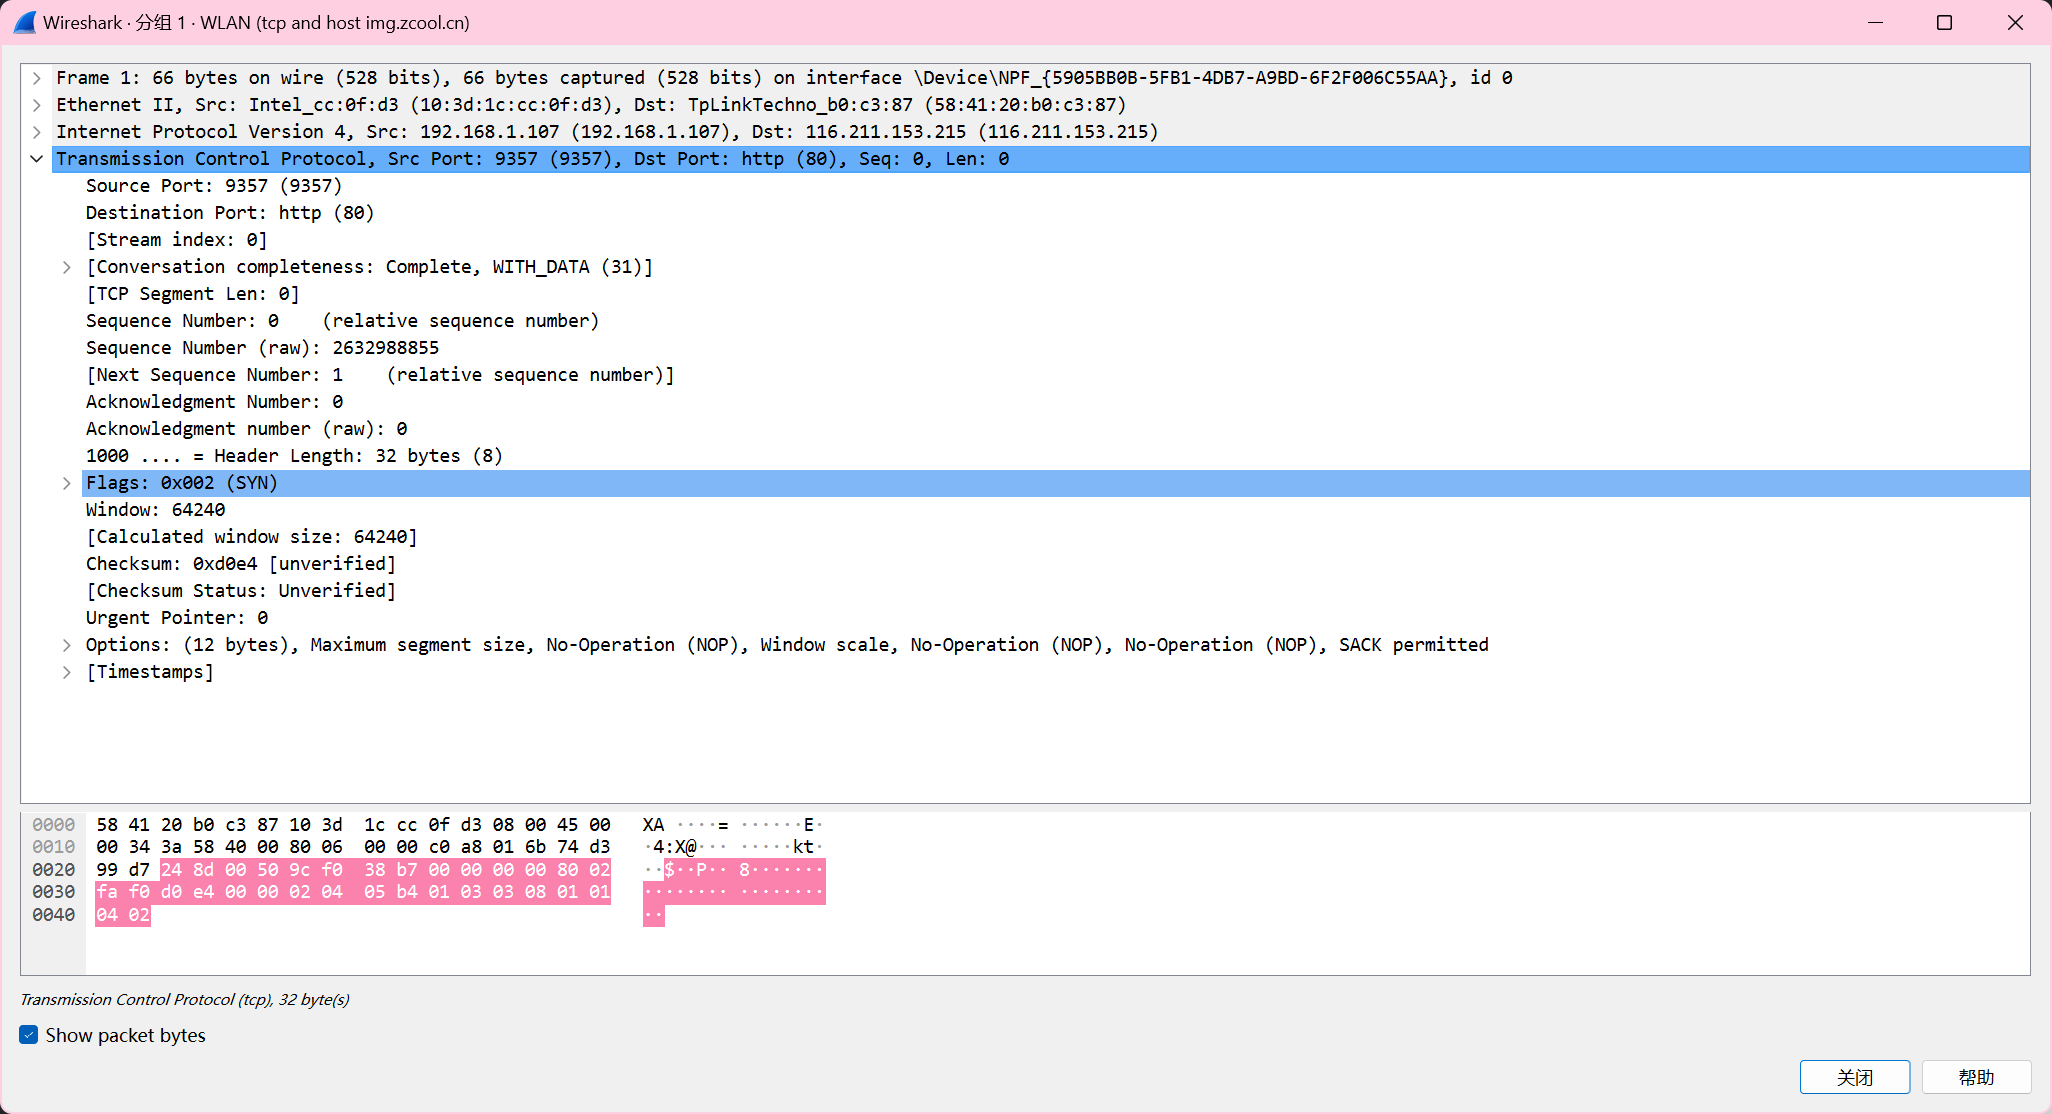
\includegraphics[width=0.79\textwidth]{img/5.png}
  \caption{一个\texttt{TCP}数据包}
\end{figure}

可以画出\texttt{TCP}包的结构如下:

% 八列的表格
\begin{table}[H]
  \centering
  \begin{tabularx}{0.8\textwidth}{|*{4}{X|}}
    \hline
    \multicolumn{2}{|X|}{源端口 Source Port}     & \multicolumn{2}{X|}{目的端口 Destination Port}                                          \\
    \multicolumn{2}{|X|}{2 bytes}                & \multicolumn{2}{X|}{2 bytes}                                                            \\
    \hline
    \multicolumn{4}{|X|}{序列号 Sequence Number}                                                                                           \\
    \multicolumn{4}{|X|}{4 bytes}                                                                                                          \\
    \hline
    \multicolumn{4}{|X|}{确认号 Acknowledgment Number}                                                                                     \\
    \multicolumn{4}{|X|}{4 bytes}                                                                                                          \\
    \hline
    \multicolumn{1}{|X|}{头部长度 Header Length} & \multicolumn{1}{X|}{标志 Flags}                & \multicolumn{2}{X|}{窗口大小 Window}   \\
    \multicolumn{2}{|X|}{共 2 bytes}             & \multicolumn{2}{X|}{2 bytes}                                                            \\
    \hline
    \multicolumn{2}{|X|}{校验和 Checksum}        & \multicolumn{2}{X|}{紧急指针 Urgent Pointer}                                            \\
    \multicolumn{2}{|X|}{2 bytes}                & \multicolumn{2}{X|}{2 bytes}                                                            \\
    \hline
    \multicolumn{4}{|X|}{可选项 Options}                                                                                                   \\
    \multicolumn{4}{|X|}{0-40 bytes}                                                                                                       \\
    \hline
                                                 &                                                &                                      & \\
    \hline
    \multicolumn{4}{|X|}{负载 Payload}                                                                                                     \\
    \multicolumn{4}{|X|}{n bytes}                                                                                                          \\
    \hline
  \end{tabularx}
  \caption{\texttt{UDP}包结构}
\end{table}

其中 \texttt{Flags} 字段包括 \texttt{Reserved}, \texttt{Accurate ECN}, \texttt{Congestion Window Reduced}, \texttt{ECN-Echo}, \\ \texttt{Urgent}, \texttt{Acknowledgment}, \texttt{Push}, \texttt{Reset}, \texttt{Syn}, \texttt{Fin}。


\texttt{TCP}数据包头部各字段的含义如下:

\begin{itemize}[noitemsep]
  \item 源端口:源端口号,占2字节,用来标识源主机的应用程序进程。
  \item 目的端口:目的端口号,占2字节,用来标识目的主机的应用程序进程。
  \item 序列号:占4字节,用来标识从TCP源端向目的端发送的字节流,发起方发送数据时对此进行标记。
  \item 确认号:占4字节,只有ACK标志位为1时,确认号字段才有效,确认号等于上次接收到的字节序号加1。
  \item 头部长度:占1字节,指示TCP头部长度。
  \item 标志:与头部长度合占2字节。各标志位的含义如下:
        \begin{itemize}[noitemsep]
          \item Reserved:保留位。
          \item Accurate ECN:显式拥塞通知。
          \item Congestion Window Reduced:拥塞窗口减小。
          \item ECN-Echo:显式拥塞通知回显。
          \item URG:紧急指针(urgent pointer)有效。
          \item ACK:确认序号有效。
          \item PSH:接收方应该尽快将这个报文交给应用层。
          \item RST:重置连接。
          \item SYN:发起一个新连接。
          \item FIN:释放一个连接。
        \end{itemize}
  \item 窗口大小:占2字节,窗口大小是指发送方在收到确认前允许发送的字节数。
  \item 校验和:占2字节,检验TCP首部和TCP数据的正确性。
  \item 紧急指针:占2字节,仅当URG标志为1时,紧急指针才有效。紧急指针告诉系统此报文段中有紧急数据,紧急数据的字节数由紧急指针指出。
  \item 可选项:占0-40字节,可选项可以有0个或多个,用于一些可选的设置。
\end{itemize}

\subsection{\texttt{TCP} 连接的建立和释放}

\subsubsection{三次握手}

我们知道,三次握手的过程如下:

\begin{enumerate}[noitemsep]
  \item 客户端发送一个\texttt{SYN}包给服务器,然后等待应答。
  \item 服务器端回应给客户端一个\texttt{ACK=1}、\texttt{SYN=1}的\texttt{TCP}数据段。
  \item 客户必须再次回应服务器端一个\texttt{ACK}确认数据段。
\end{enumerate}

在 \texttt{Wireshark} 中,我们可以看到三次握手的过程如下:

\begin{figure}[H]
  \centering
  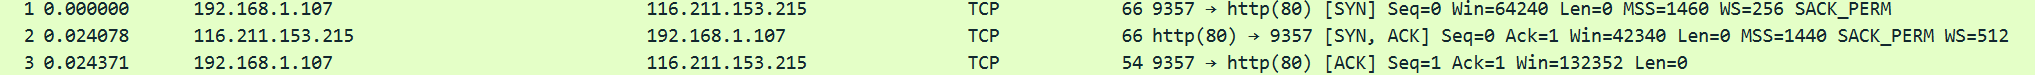
\includegraphics[width=0.95\textwidth]{img/6.png}
  \caption{三次握手}
\end{figure}

画出三次握手协议的步骤图如下:

\begin{figure}[H]
  \centering
  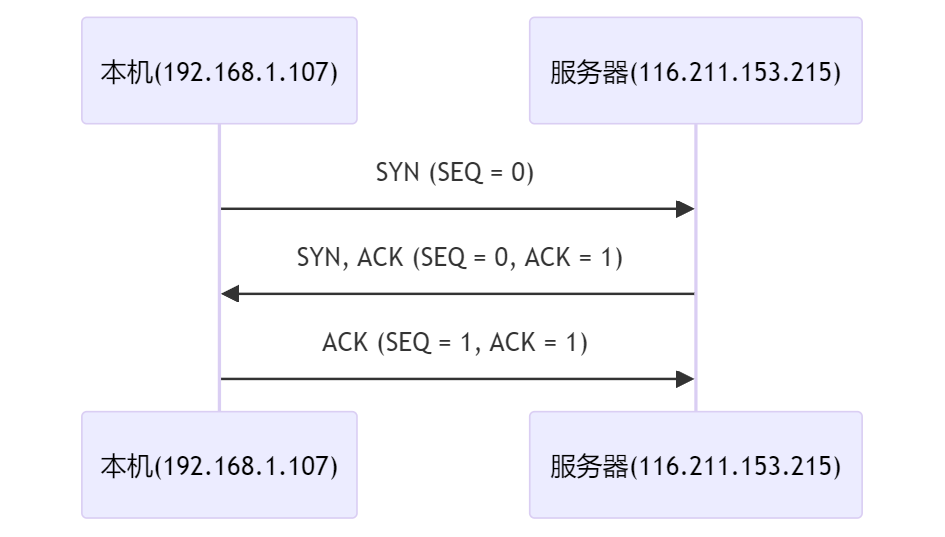
\includegraphics[width=0.95\textwidth]{img/7.png}
  \caption{三次握手协议的步骤图}
\end{figure}

\subsubsection{四次挥手}

TCP的四次挥手主要分为以下四个步骤:

\begin{enumerate}[noitemsep]
  \item 客户端进程发出断开连接指令,这将导致客户端的\texttt{TCP}程序创建一个特殊的\texttt{TCP}报文段,发送到服务器。这个报文段的\texttt{FIN}字段被置为1,表示这是一条断开连接的报文;
  \item 服务器接收到客户端发来的断开连接报文,向客户端回送这个报文的确认报文(\texttt{ACK}字段为1),告诉服务器已经接收到\texttt{FIN}报文,并允许断开连接;
  \item 服务器发送完确认报文后,服务器的\texttt{TCP}程序创建一条自己的断开连接报文,此报文的\texttt{FIN}字段被置为1,然后发往客户端;
  \item 客户端接收到服务器发来的\texttt{FIN}报文段,则产生一条确认报文(\texttt{ACK}为1),发送给服务器,告知服务器已经接收到了它的断开报文。服务器接收到这条\texttt{ACK}报文段后,释放\texttt{TCP}连接相关的资源(缓存和变量),而客户端等待一段时间后(半分钟、一分钟或两分钟),也释放处于客户端的缓存和变量。
\end{enumerate}

在 \texttt{Wireshark} 中,我们可以看到四次挥手的过程如下:

\begin{figure}[H]
  \centering
  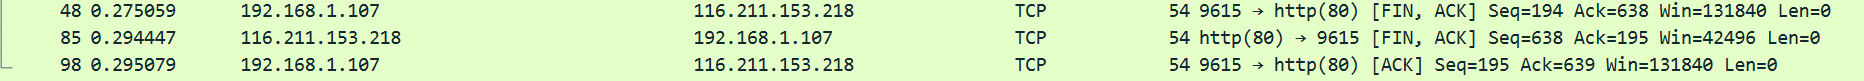
\includegraphics[width=0.95\textwidth]{img/8.png}
  \caption{四次挥手}
\end{figure}

画出四次挥手协议的步骤图如下:

\begin{figure}[H]
  \centering
  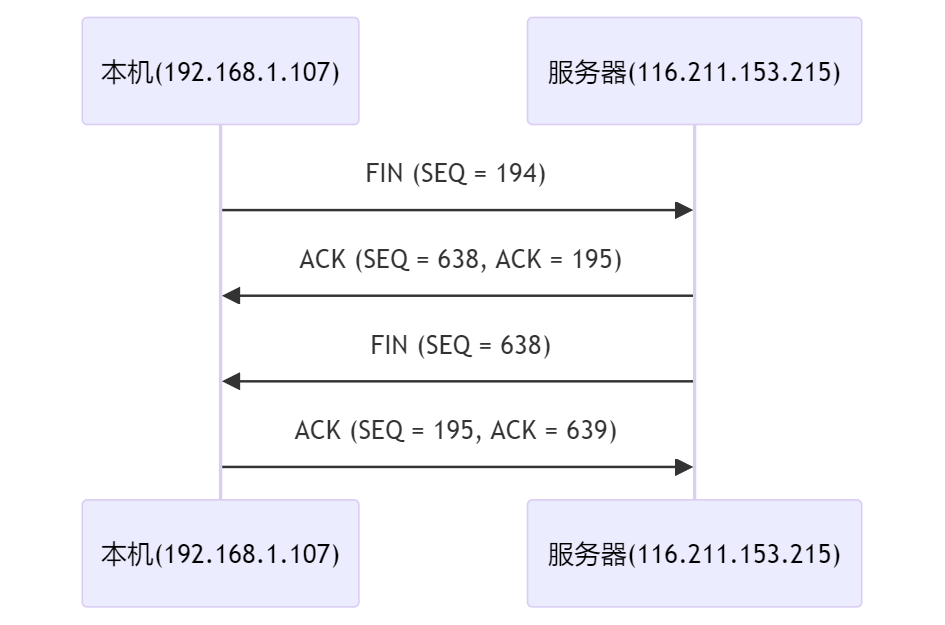
\includegraphics[width=0.95\textwidth]{img/9.png}
  \caption{四次挥手协议的步骤图}
\end{figure}

回答问题:

\begin{itemize}[noitemsep]
  \item 思考为什么连接的时候是三次握手,关闭的时候却是四次挥手?

        因为一方在收到对方发来的\texttt{FIN}包时,有可能还有未发送完的数据包,所以这时它会先给对方发送一个\texttt{ACK}包,等它将数据包都处理完毕并发送后,再向对方发送\texttt{FIN ACK}报文来同意关闭连接,最后对方收到\texttt{FIN ACK}包,向它回复\texttt{ACK}包。而建立连接时,不会出现这个问题,所以只需要三次握手即可建立连接。

\end{itemize}

\subsection{TCP 数据传输}

观察 \texttt{Wireshark} 生成的 \texttt{IO} 图表, 如下所示:

\begin{figure}[H]
  \centering
  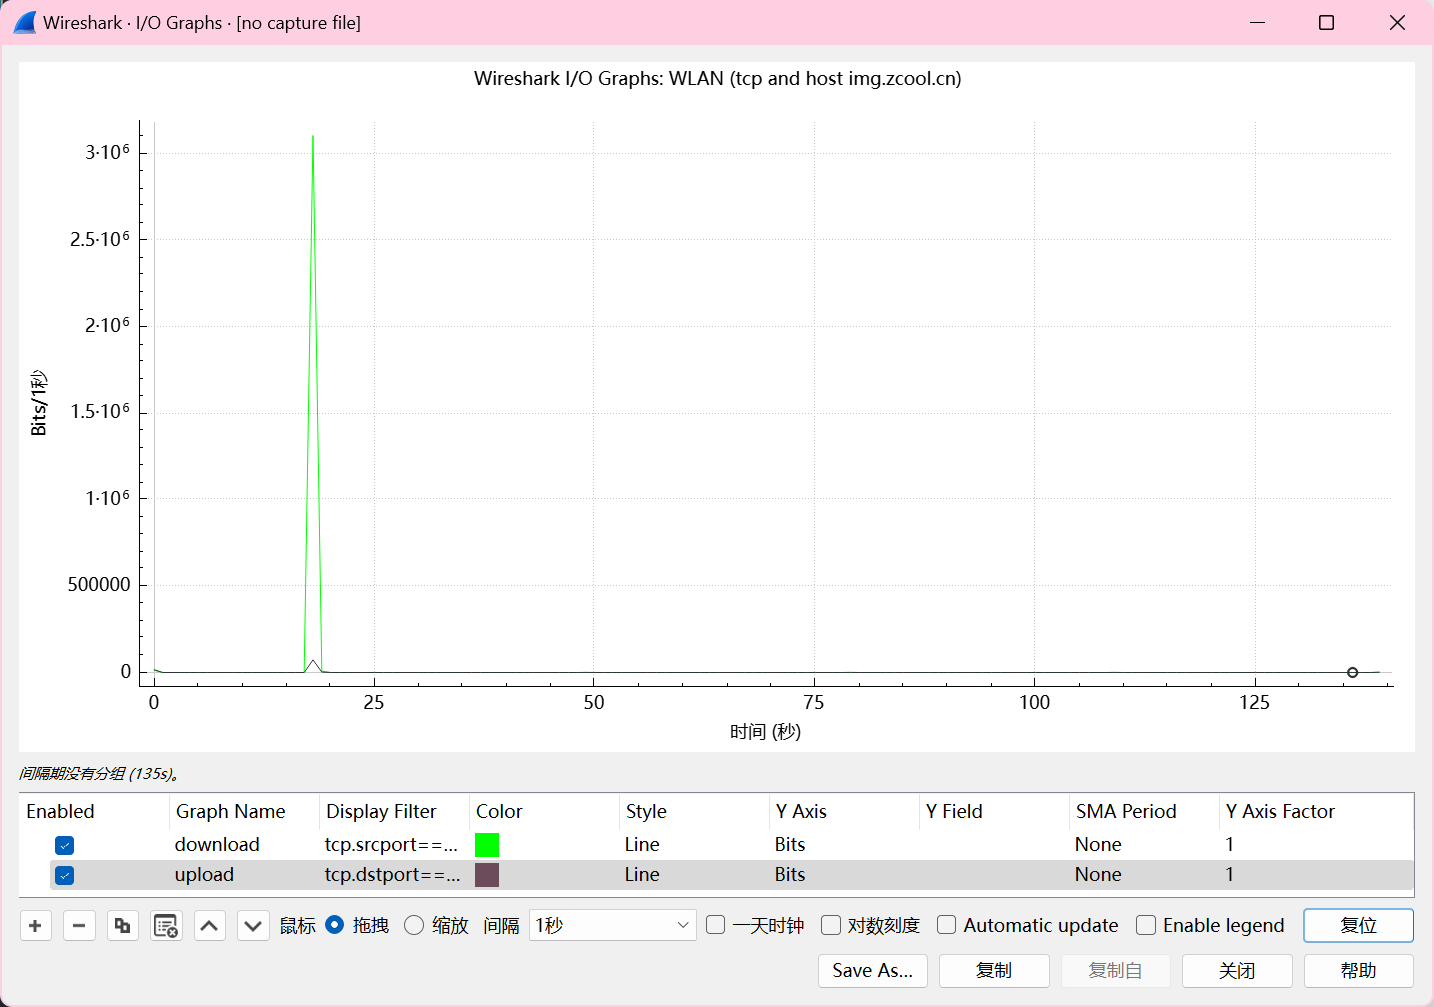
\includegraphics[width=0.95\textwidth]{img/10.png}
  \caption{\texttt{IO} 图表}
\end{figure}

下载速度为 \texttt{3107000 Bits/s},
上传速度为 \texttt{732900 Bits/s}

~\\
观察数据包传输过程,回答问题:

\begin{itemize}[noitemsep]
  \item 观察数据传输过程中 \texttt{Acknowledgment number},\texttt{sequence number} 和 \texttt{Segment Len} 之间的变化

  \item 如果最近从服务器收到的 \texttt{TCP} 数据段的序列号是 $X$,那么下一个发送的 \texttt{ACK} 是多少?

        下一个发送的 \texttt{ACK} 是 $X + \texttt{Segment Len}$

\end{itemize}

\subsection{问题讨论}

下载一个大文件,观察 \texttt{TCP} 流图表,如下所示:

\begin{figure}[H]
  \centering
  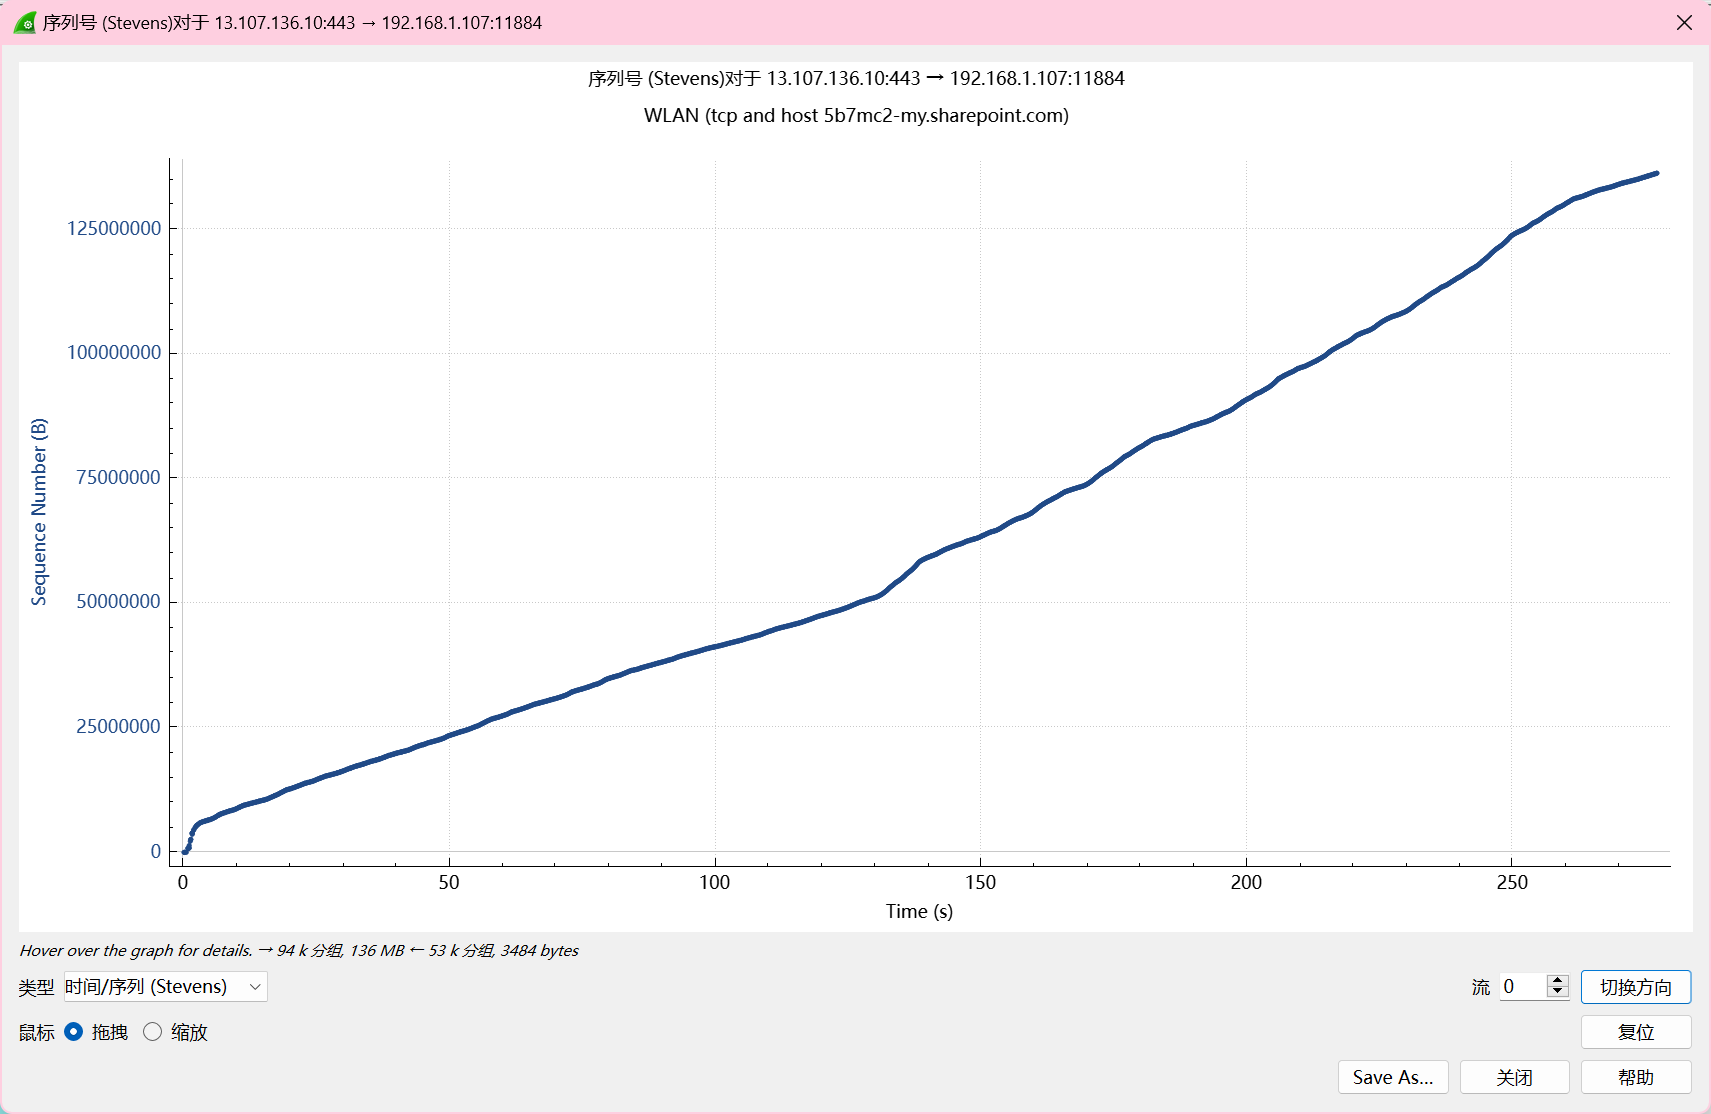
\includegraphics[width=0.8\textwidth]{img/11.png}
  \caption{序列号}
\end{figure}

\begin{figure}[H]
  \centering
  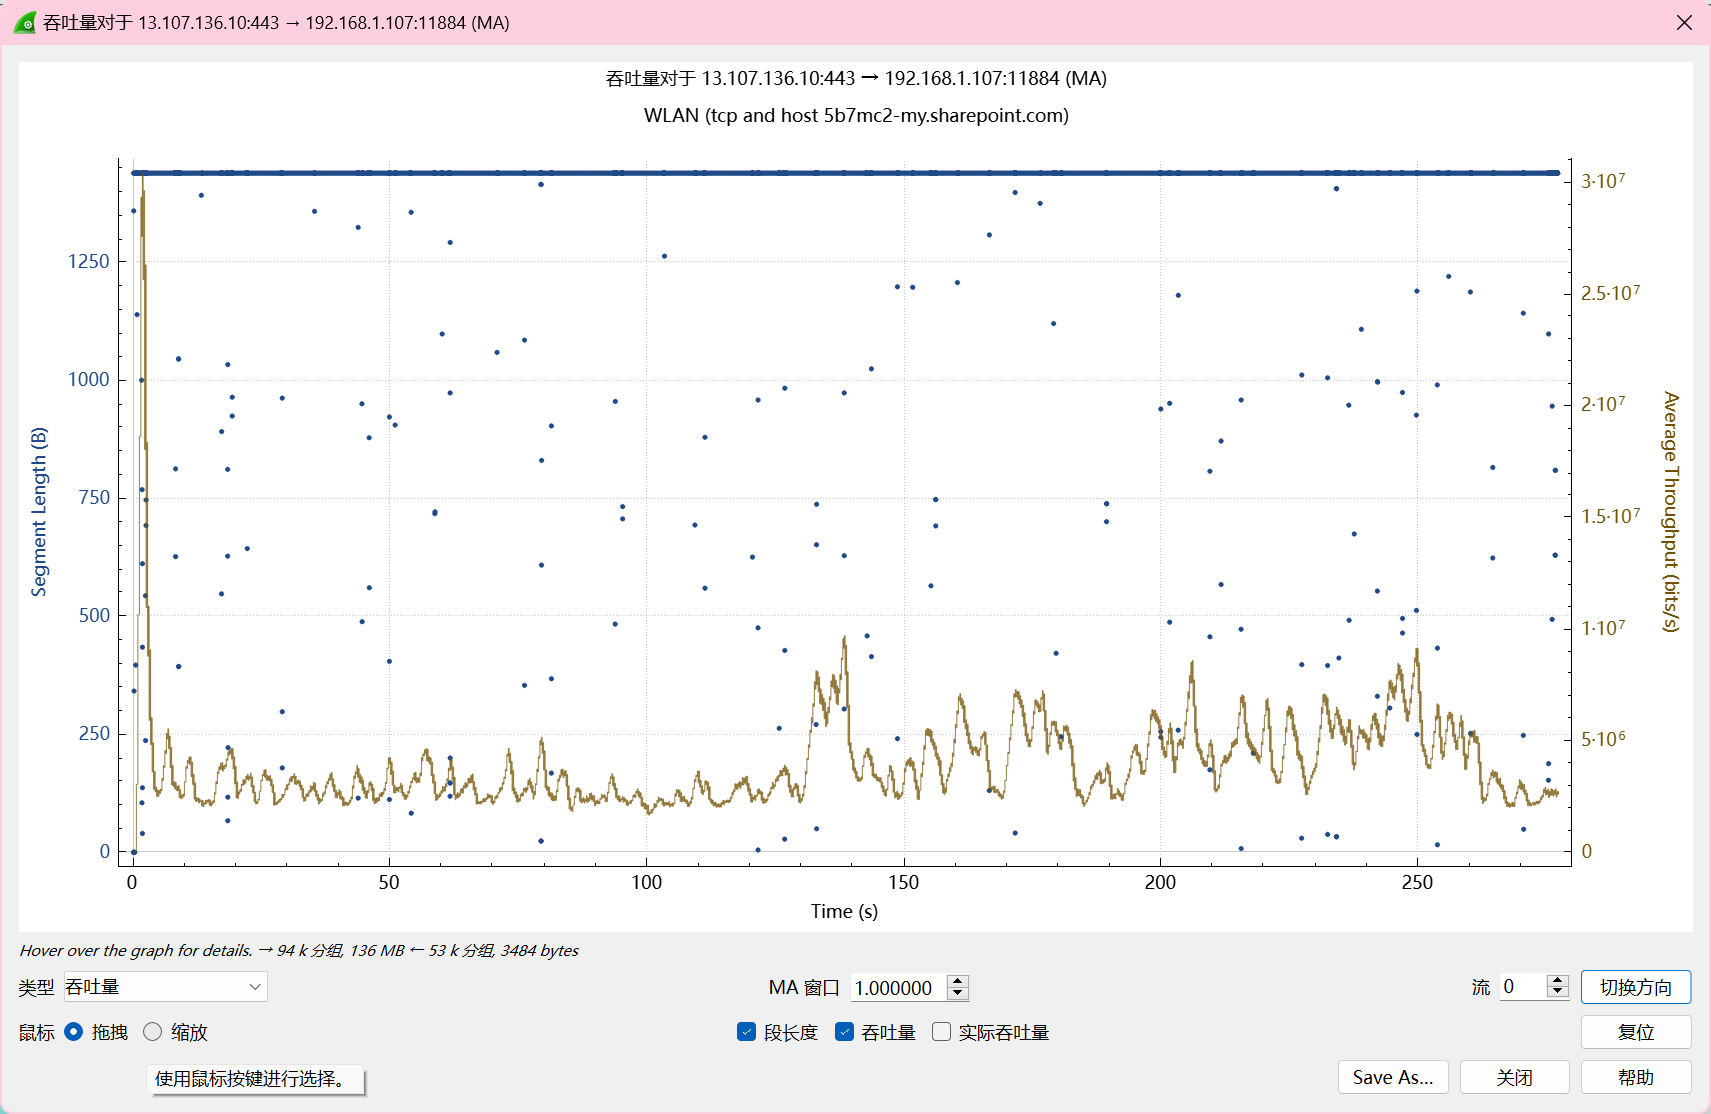
\includegraphics[width=0.8\textwidth]{img/12.png}
  \caption{吞吐量}
\end{figure}

\begin{figure}[H]
  \centering
  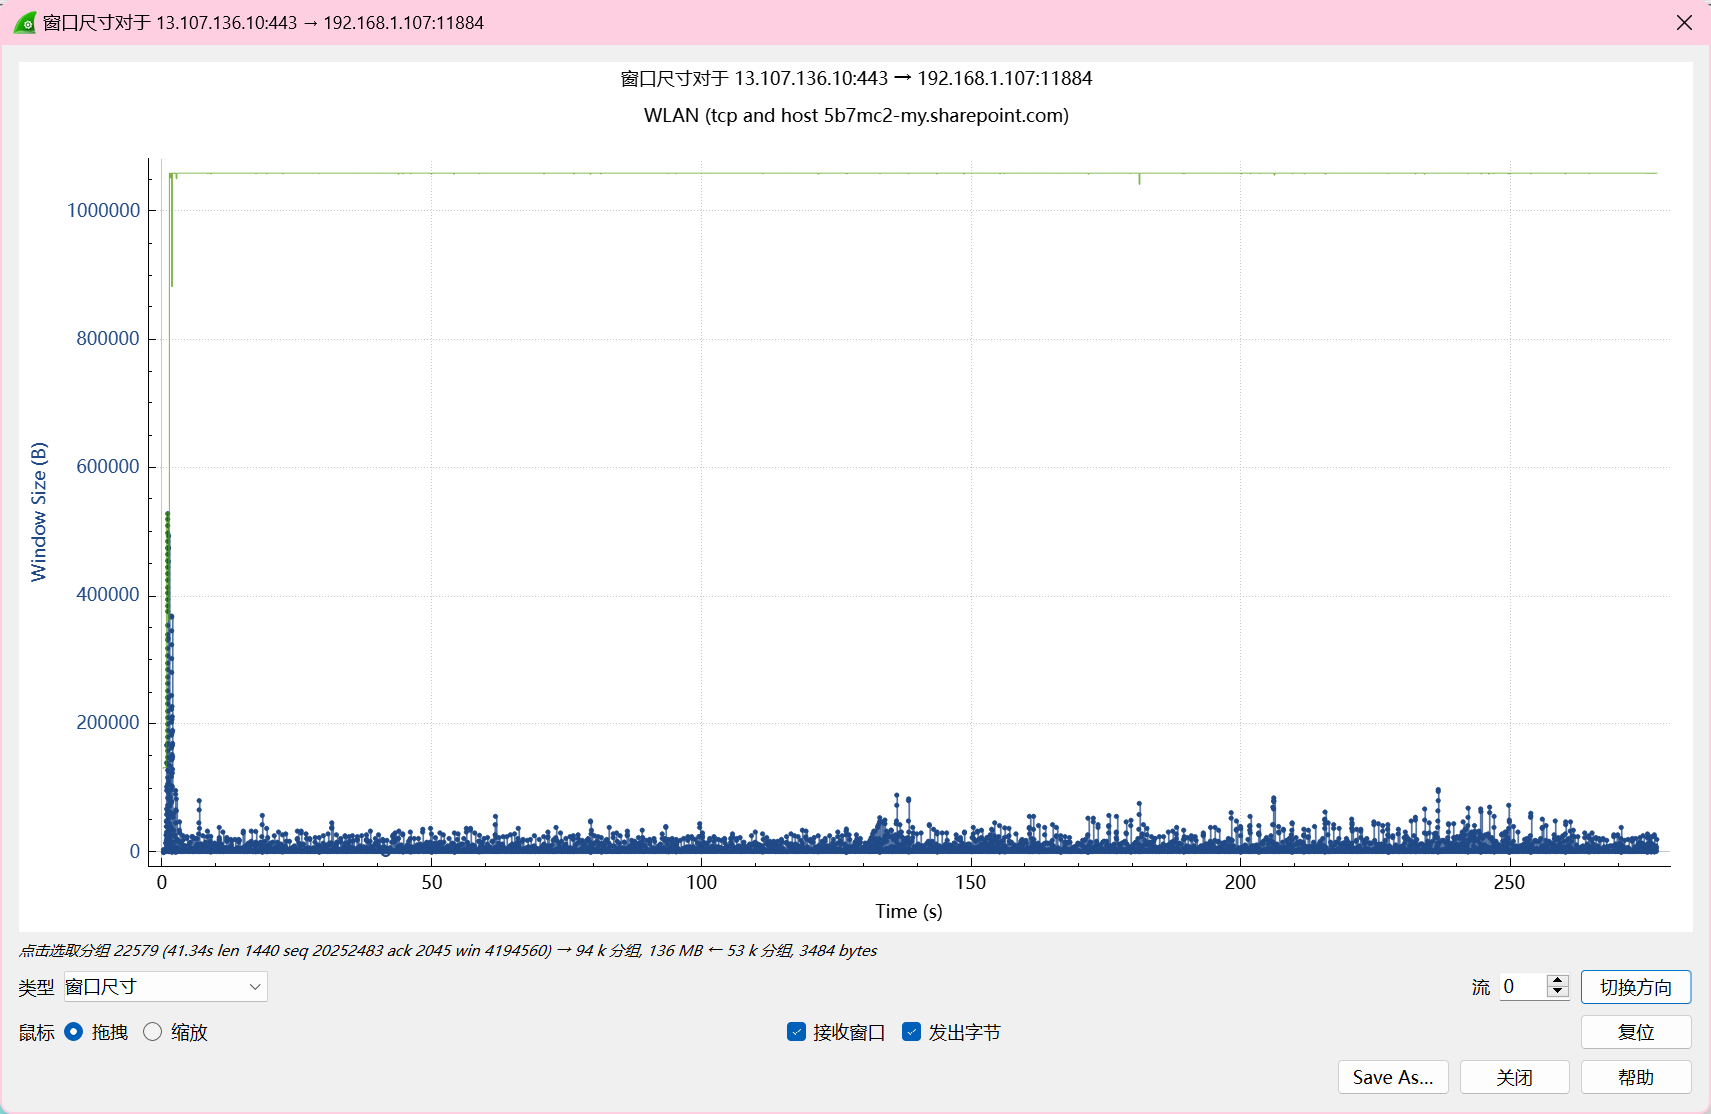
\includegraphics[width=0.8\textwidth]{img/13.png}
  \caption{窗口尺寸}
\end{figure}

\begin{figure}[H]
  \centering
  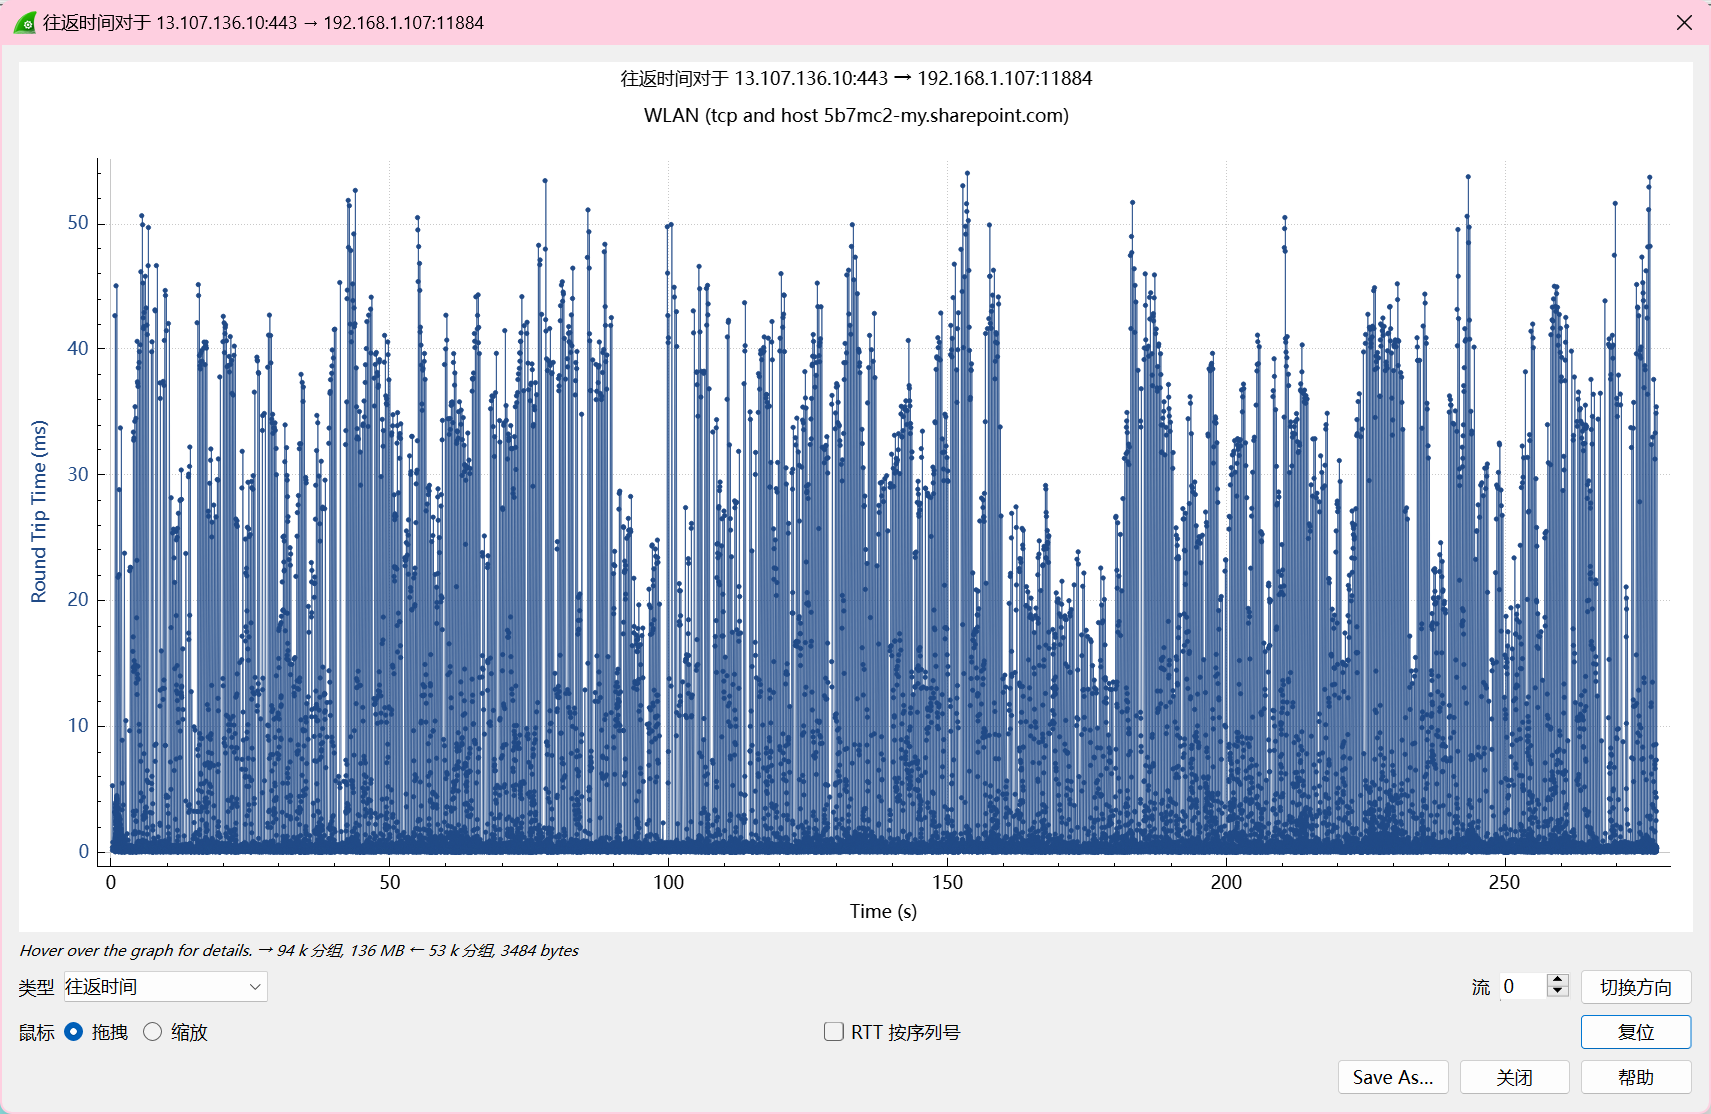
\includegraphics[width=0.8\textwidth]{img/14.png}
  \caption{往返时间}
\end{figure}

回答下列问题:

\begin{itemize}[noitemsep]
  \item Explore the congestion control and the classic AIMD behavior of TCP. To do this, you will likely want to capture a trace while you are sending (not receiving) a moderate amount of data on a TCP connection. You can then use the “TCP Stream Graph” tools as well as other analysis to observe how the congestion window changes over time.
        从吞吐量图表中可以看出,吞吐量随着时间的增加而增加,但是在某些时刻会突然下降,不断波动,这是因为在这些时刻发生了拥塞,\texttt{TCP} 会减小拥塞窗口,然后再慢慢增加,这就是拥塞控制的过程。
  \item Explore the reliability mechanisms of TCP more deeply. Capture a trace of a connection that includes segment loss. See what triggers the retransmissions and when. Also look at the round-trip time estimator.

        可以看到,当接受到的数据包顺序错误时(可能是之前的数据包丢失了),会触发重传机制,重传丢失的数据包。

        \begin{figure}[H]
          \centering
          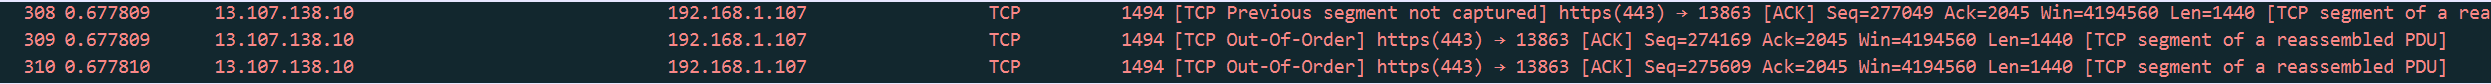
\includegraphics[width=0.95\textwidth]{img/15.png}
          \caption{错误重传}
        \end{figure}

        往返时间图表已在上方列出。
  \item Look at the use of options including SACK to work through the details. You should see information about ranges of received bytes during times of segment loss.

        观察一个 \texttt{Options} 中包含了 \texttt{SACK} 的数据包,如下图所示:

        \begin{figure}[H]
          \centering
          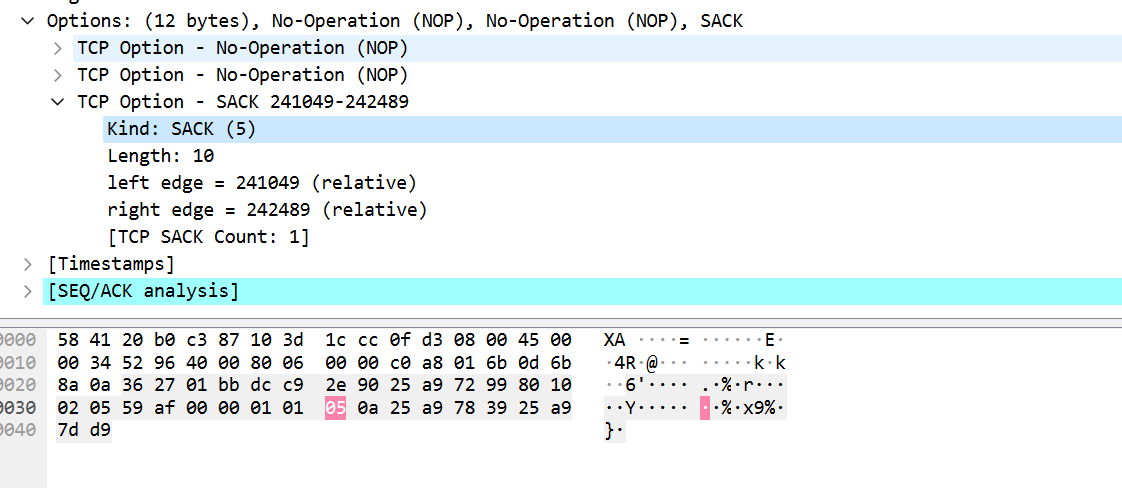
\includegraphics[width=0.8\textwidth]{img/16.png}
          \caption{\texttt{SACK}}
        \end{figure}

        可以看到,\texttt{SACK} 中包含了丢失的数据包的序列号范围。
  \item TCP is the transport layer underlying the web. You can see how your browser makes use of TCP by setting up concurrent connections.

        浏览器处理用户请求时,会建立多个 \texttt{TCP} 连接,并发地处理用户请求。

\end{itemize}

\section{实验结果总结}

在本次实验中,我学习了 \texttt{TCP} 的数据包结构,以及 \texttt{TCP} 连接建立和释放的过程,还学习了 \texttt{TCP} 数据传输的过程。

同时,我还了解到了 \texttt{TCP} 的拥塞控制机制,以及 \texttt{TCP} 的可靠性机制。

\section{附录}

无

\end{document}